%!TEX root = vorlage.tex

\clearpage\onecolumn
\begin{appendices}
\section{Tables}

\begin{table}[ht]
    \centering
    \begin{tabular}{llrr}
    \toprule
    ~                & ~ & \multicolumn{2}{c}{\textbf{Predicted class}}\\
    ~                & ~ & \multicolumn{1}{c}{\textbf{0}} & \multicolumn{1}{c}{\textbf{1}} \\% \cmidrule{3-4}
    \textbf{Actual}  & \multicolumn{1}{c}{\textbf{0}} & \num{38640407}  & \num{2654875} \\
    \textbf{class}   & \multicolumn{1}{c}{\textbf{1}} &   \num{408816}  & \num{1303902} \\ \bottomrule
    \end{tabular}
    \caption{Confusion matrix of a model trained soley on pixel colors.
             Class~0 is background, class~1 is medical instruments.}
    \label{table:cm-model-301}
\end{table}

\begin{table}[ht]
    \centering
    \begin{tabular}{llrr}
    \toprule
    ~                & ~ & \multicolumn{2}{c}{\textbf{Predicted class}}\\
    ~                & ~ & \multicolumn{1}{c}{\textbf{0}} & \multicolumn{1}{c}{\textbf{1}} \\% \cmidrule{3-4}
    \textbf{Actual}  & \multicolumn{1}{c}{\textbf{0}} & \num{38989042}  & \num{3780484} \\
    \textbf{class}   & \multicolumn{1}{c}{\textbf{1}} &    \num{60181}  &  \num{178293} \\ \bottomrule
    \end{tabular}
    \caption{Confusion matrix of a model trained soley on pixel colors. Additionally,
             a morphological closing operation with $\SI{3}{\pixel}$ was applied.
             Class~0 is background, class~1 is medical instruments.}
    \label{table:cm-model-301-closing}
\end{table}

\begin{table}[ht]
    \centering
    \begin{tabular}{llrr}
    \toprule
    ~                & ~ & \multicolumn{2}{c}{\textbf{Predicted class}}\\
    ~                & ~ & \multicolumn{1}{c}{\textbf{0}} & \multicolumn{1}{c}{\textbf{1}} \\% \cmidrule{3-4}
    \textbf{Actual}  & \multicolumn{1}{c}{\textbf{0}} & \num{38541570}  & \num{2284099} \\
    \textbf{class}   & \multicolumn{1}{c}{\textbf{1}} &   \num{507653}  & \num{1674678} \\ \bottomrule
    \end{tabular}
    \caption{Confusion matrix of a model trained on pixel colors and the pixels coordinates. Additionally, a morphological closing operation was applied.
             Class~0 is background, class~1 is medical instruments.}
    \label{table:cm-model-303}
\end{table}

\begin{table}[ht]
    \centering
    \begin{tabular}{lrrr}
    \toprule
    \textbf{Model}        & \textbf{Accuracy} & \textbf{Precision} & \textbf{Recall}   \\ \midrule
    Baseline              & 92.88 \%          & 76.13 \%         & 32.94 \% \\
                          & {\tiny (+8 \%)}   & {\tiny (+4 \%)}  & {\tiny (+11 \%)}\\
    Local model + opening & 93.42 \%          & 76.98 \%         & 40.65 \% \\
                          & {\tiny (+62 \%)}  & {\tiny (+41 \%)} & {\tiny (+77 \%)}\\
    FCN                   & \textbf{97.32} \% & \textbf{85.87} \%& 84.90 \% \\ \midrule
    KIT                   & 93 \%             & 69 \%            & 46 \% \\
    Lausanne              & 96.5 \%           & 76 \%            & \textbf{93} \% \\
    \bottomrule
    \end{tabular}
    \caption{Results of the Endoscopic Vision Challenge \enquote{EndoVis}}
    \label{table:challenge-results}
\end{table}

\clearpage
\section{Graphs}
\begin{figure}[ht]
    \centering
    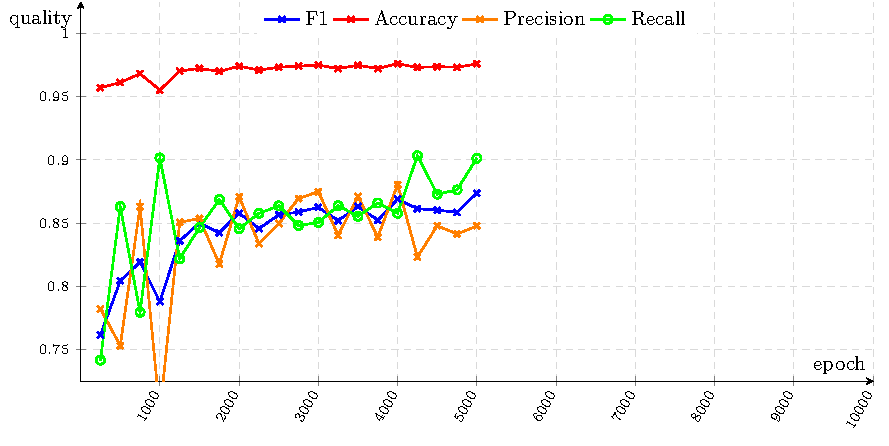
\includegraphics[width=\linewidth]{csv-line-plot/5000-no-augmentation.pdf}
    \caption{Training without data augmentation}
    \label{fig:graph-training-no-augmentation}
\end{figure}

\begin{figure}[ht]
    \centering
    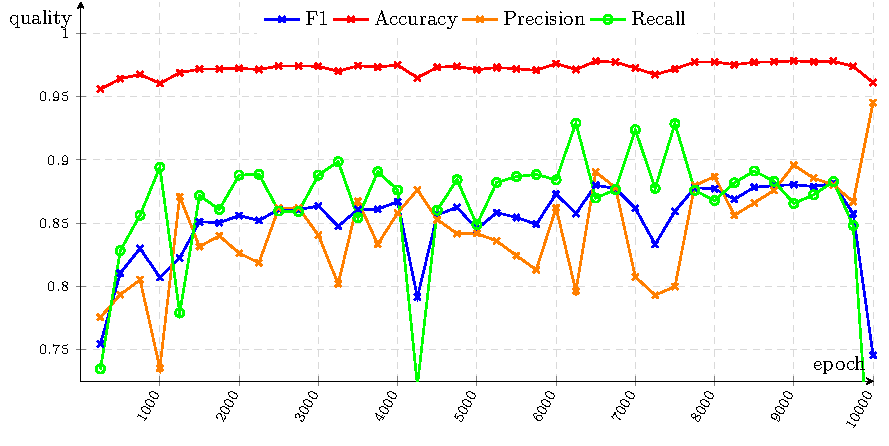
\includegraphics[width=\linewidth]{csv-line-plot/10000-no-augmentation.pdf}
    \caption{Training without data augmentation}
    \label{fig:graph-training-no-augmentation}
\end{figure}

\begin{figure}[ht]
    \centering
    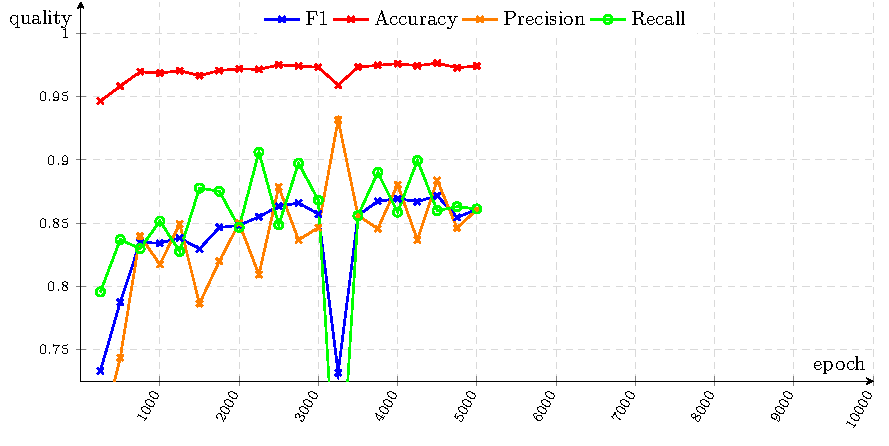
\includegraphics[width=\linewidth]{csv-line-plot/5000-lr-flip.pdf}
    \caption{Training with data augmentation (left-right flip)}
    \label{fig:graph-training-lr-flip}
\end{figure}

\begin{figure}[ht]
    \centering
    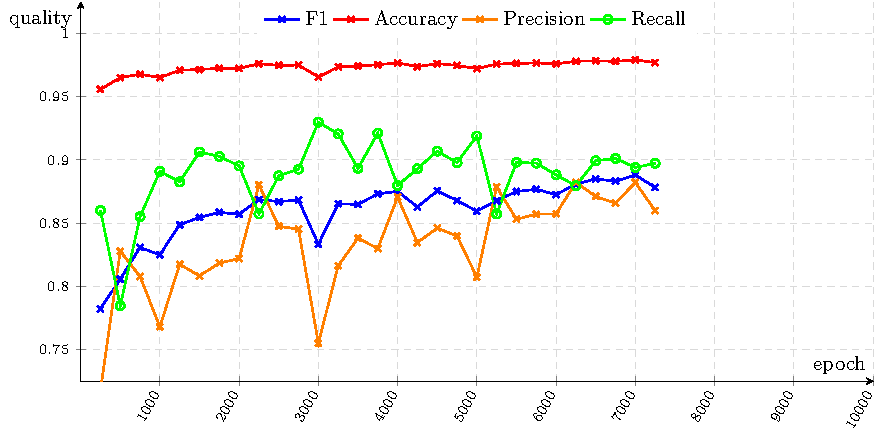
\includegraphics[width=\linewidth]{csv-line-plot/5xxx-ud-flip.pdf}
    \caption{Training with data augmentation (up-down flip)}
    \label{fig:graph-training-ud-flip}
\end{figure}

\begin{figure}[ht]
    \centering
    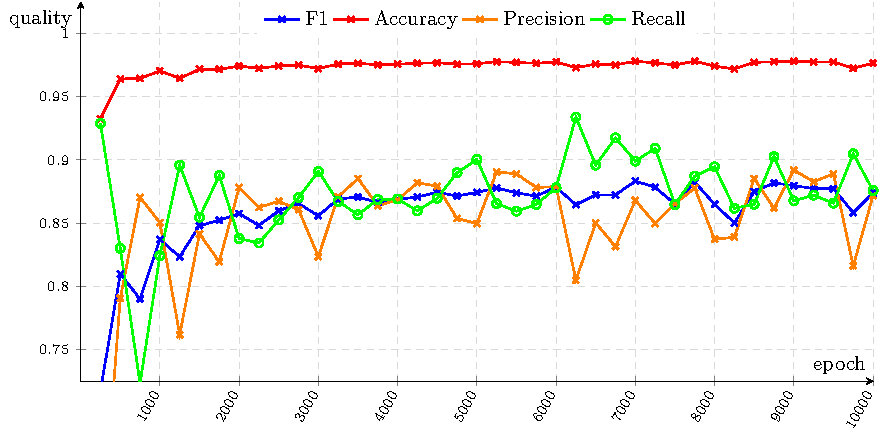
\includegraphics[width=\linewidth]{csv-line-plot/10000-random-brightnes.pdf}
    \caption{Training with data augmentation (random brightness)}
    \label{fig:graph-training-ud-flip}
\end{figure}

\begin{figure}[ht]
    \centering
    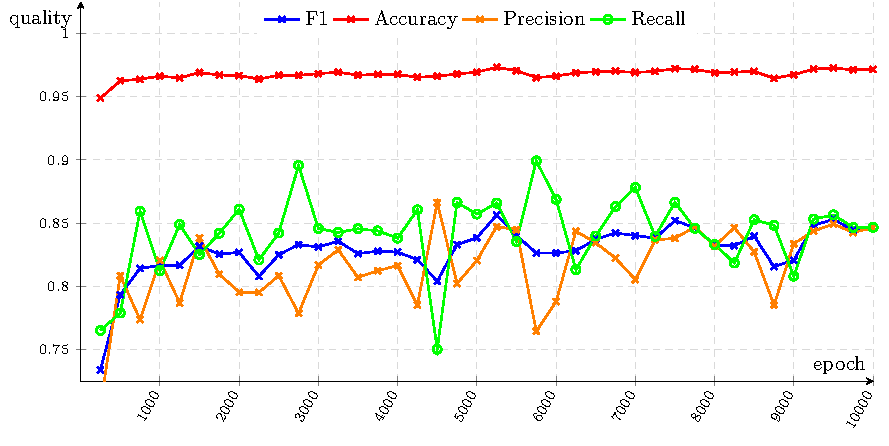
\includegraphics[width=\linewidth]{csv-line-plot/10000-random-crops.pdf}
    \caption{Training with data augmentation (random crops)}
    \label{fig:graph-training-ud-flip}
\end{figure}

\begin{figure}[ht]
    \centering
    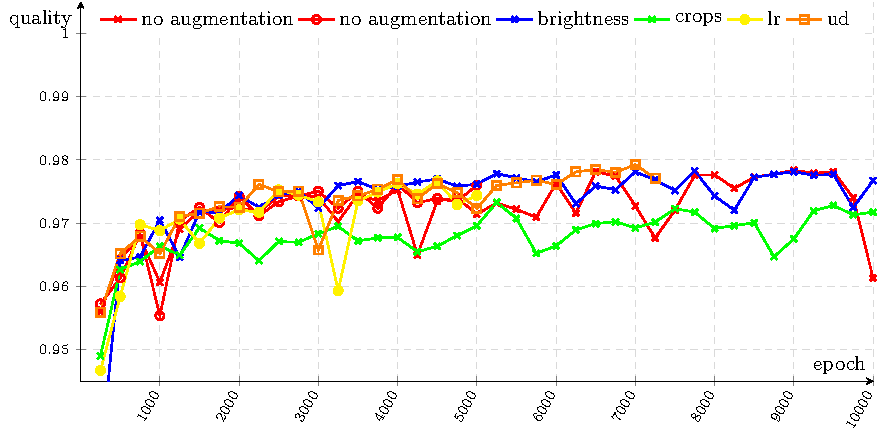
\includegraphics[width=\linewidth]{csv-line-plot/accuracy-all.pdf}
    \caption{Accuracy over epochs of FCNs with different data augmentation
             setups. No augmentation was evaluated twice with different
             random initialization, random brightness and random crops as
             well as upside down flips and left-right flips.}
    \label{fig:graph-accuracy-all}
\end{figure}


\begin{figure}[ht]
    \centering
    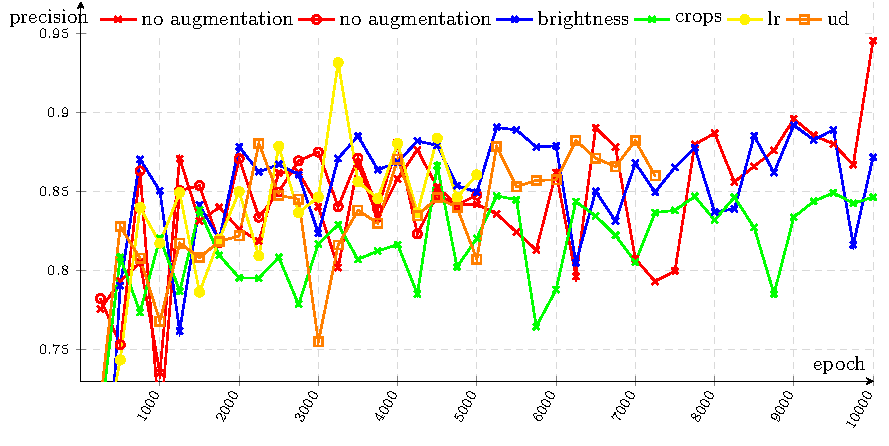
\includegraphics[width=\linewidth]{csv-line-plot/precision-all.pdf}
    \caption{Precision over epochs of FCNs with different data augmentation
             setups. No augmentation was evaluated twice with different
             random initialization, random brightness and random crops as
             well as upside down flips and left-right flips.}
    \label{fig:graph-precision-all}
\end{figure}


\begin{figure}[ht]
    \centering
    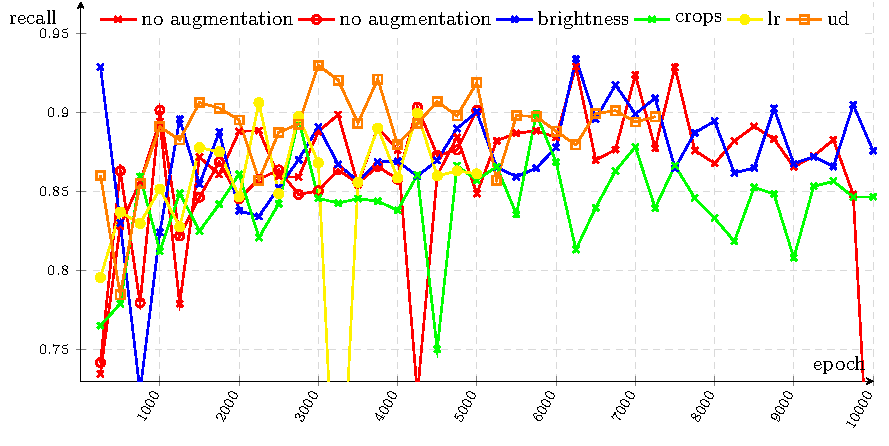
\includegraphics[width=\linewidth]{csv-line-plot/recall-all.pdf}
    \caption{Recall over epochs of FCNs with different data augmentation
             setups. No augmentation was evaluated twice with different
             random initialization, random brightness and random crops as
             well as upside down flips and left-right flips.}
    \label{fig:graph-recall-all}
\end{figure}


\end{appendices}
